% Update slides, version 4 (24 Nov 2026):
%   1. choice of the linear iterative method: serial comparison of five
%      solvers on dumped L2 systems (iface/TestKineticSolversSerial.cpp)
%   2. memory and time scaling in toroidal geometry, L1, Nr = 44:
%      job 2900942 on Pitagora, figures in v4_2900942/ (memory_scaling.png and
%      memory_time_breakdown.png from summarize_memory.py)
% Include with % Update slides, version 4 (24 Nov 2026):
%   1. choice of the linear iterative method: serial comparison of five
%      solvers on dumped L2 systems (iface/TestKineticSolversSerial.cpp)
%   2. memory and time scaling in toroidal geometry, L1, Nr = 44:
%      job 2900942 on Pitagora, figures in v4_2900942/ (memory_scaling.png and
%      memory_time_breakdown.png from summarize_memory.py)
% Include with % Update slides, version 4 (24 Nov 2026):
%   1. choice of the linear iterative method: serial comparison of five
%      solvers on dumped L2 systems (iface/TestKineticSolversSerial.cpp)
%   2. memory and time scaling in toroidal geometry, L1, Nr = 44:
%      job 2900942 on Pitagora, figures in v4_2900942/ (memory_scaling.png and
%      memory_time_breakdown.png from summarize_memory.py)
% Include with % Update slides, version 4 (24 Nov 2026):
%   1. choice of the linear iterative method: serial comparison of five
%      solvers on dumped L2 systems (iface/TestKineticSolversSerial.cpp)
%   2. memory and time scaling in toroidal geometry, L1, Nr = 44:
%      job 2900942 on Pitagora, figures in v4_2900942/ (memory_scaling.png and
%      memory_time_breakdown.png from summarize_memory.py)
% Include with \input{update_frames_v4} (update_2026-11-24.tex).

% =====================================================================
% Part 1: linear solver
% =====================================================================
\begin{frame}{Linear solver comparison: setup}
    \small
    \begin{itemize}
        \item kinetic system dumped by \texttt{dreami} (\texttt{-dream\_save\_system}), L2, cylindrical
        \begin{itemize}
            \item $N = 1.67$\,M unknowns, $11.4$\,M nonzeros
            \item $N_r = 11$ radii, $152\,000$ rows per radius ($f_\mathrm{hot}$ $32\,000$ + $f_\mathrm{re}$ $120\,000$)
        \end{itemize}
        \item two snapshots
        \begin{itemize}
            \item injection end ($\Delta t = 1.8\times10^{-7}$\,s, the source step)
            \item current quench at 29\,ms, $E \approx 31$\,V/m, with
                  $\Delta t = 1.0\times10^{-7}$\,s, the DREAM substep of V.~Svensson's coupled runs
                  ($N_t = \lceil \Delta t_\mathrm{fluid} / 10^{-7}\,\mathrm{s} \rceil$),
                  instead of the source step $10^{-4}$\,s
        \end{itemize}
        \item serial, zero initial guess, restart 100, stop at $\|r\|/\|b\| < 10^{-10}$ (true residual)
        \item five solvers; ``BJ(r)'' = block Jacobi over the radius, one block per radius
        \begin{enumerate}
            \item BJ(r) + [GMRES + AMG with Euclid ILU(1) smoother] + FGMRES \quad (MIRadialBJ)
            \item BJ(r) + one AMG V-cycle + GMRES
            \item BJ(r) + ILU(0) + GMRES
            \item AMG + GMRES \quad (whole matrix)
            \item ILU(0) + GMRES \quad (whole matrix)
        \end{enumerate}
    \end{itemize}
\end{frame}

% ---------------------------------------------------------------------
\begin{frame}{Linear solver comparison: results (serial, L2)}
    \small
    \begin{center}
    \resizebox{\linewidth}{!}{%
    \begin{tabular}{l|rrr|rrr}
        \hline
        & \multicolumn{3}{c|}{injection end} & \multicolumn{3}{c}{CQ 29\,ms, $\Delta t = 10^{-7}$\,s} \\
        solver & its & time [s] & error & its & time [s] & error \\
        \hline
        \textbf{BJ(r) + [GMRES+AMG/Euclid(1)] + FGMRES} & \textbf{3} & \textbf{6.8} & $5\times10^{-12}$
                                                       & \textbf{3} & \textbf{4.7} & $4\times10^{-12}$ \\
        BJ(r) + AMG + GMRES        & 22  & 8.4  & $7\times10^{-11}$ & 221 & 41.3 & $1\times10^{-11}$ \\
        BJ(r) + ILU(0) + GMRES     & 152 & 29.4 & $1\times10^{-10}$ & 238 & 19.9 & $1\times10^{-10}$ \\
        AMG + GMRES                & 21  & 11.1 & $9\times10^{-12}$ & --  & --   & -- \\
        ILU(0) + GMRES             & 150 & 29.8 & $1\times10^{-10}$ & --  & --   & -- \\
        \hline
    \end{tabular}}
    \end{center}
    \vspace{0.3em}
    \begin{itemize}
        \item time = setup + solve; error = $\|x - x_\mathrm{ref}\| / \|x_\mathrm{ref}\|$
        \item method 1: inner GMRES at most 9 iterations per radius (99 in total), on both snapshots
        \item CQ, AMG + GMRES and ILU(0) + GMRES: out of memory on the serial partition, to be re-run
        \item true residual after ``convergence'': $\lesssim 10^{-9}$, except with AMG
              (BJ(r) + AMG: $7\times10^{-8}$, AMG: $1\times10^{-8}$)
    \end{itemize}
\end{frame}

% ---------------------------------------------------------------------
\begin{frame}{Chosen linear method}
    \begin{center}
        \textbf{FGMRES, preconditioned by block Jacobi over the radius;}\\
        \textbf{each block solved by GMRES + BoomerAMG with Euclid ILU(1) smoother}
    \end{center}
    \vspace{0.5em}
    \small
    \begin{itemize}
        \item \textbf{fewest iterations}: 3 outer iterations on both snapshots
        \item \textbf{fastest}: 4.7\,s (CQ) and 6.8\,s (injection);
              next best 19.9\,s (CQ, BJ + ILU) and 8.4\,s (injection, BJ + AMG)
        \item \textbf{robust}: BJ + one AMG V-cycle needs 22 iterations at injection but 221 in the CQ;
              method 1 needs 3 in both
        \item \textbf{parallel by construction}: one block per radius, so with up to $N_r$ ranks
              the preconditioner needs no communication; the radial coupling is left to the outer FGMRES
        \item FGMRES because the inner Krylov solve makes the preconditioner change from one iteration to the next
        \item Euclid ILU(1) rather than ILU(0): with ILU(0) the inner GMRES breaks down on
              some radii of the CQ snapshot at 29\,ms
    \end{itemize}
\end{frame}

% =====================================================================
% Part 2: memory and time scaling, toroidal geometry
% =====================================================================
\begin{frame}{Memory and speed-up test: toroidal geometry}
    \footnotesize
    4 CQ snapshots (5, 10, 20, 40\,ms), analytic toroidal geometry, L1, $N_r = 44$:
    1.67\,M unknowns, 1 time step, MIRadialBJ; same behaviour for the 4 snapshots
    \begin{center}
        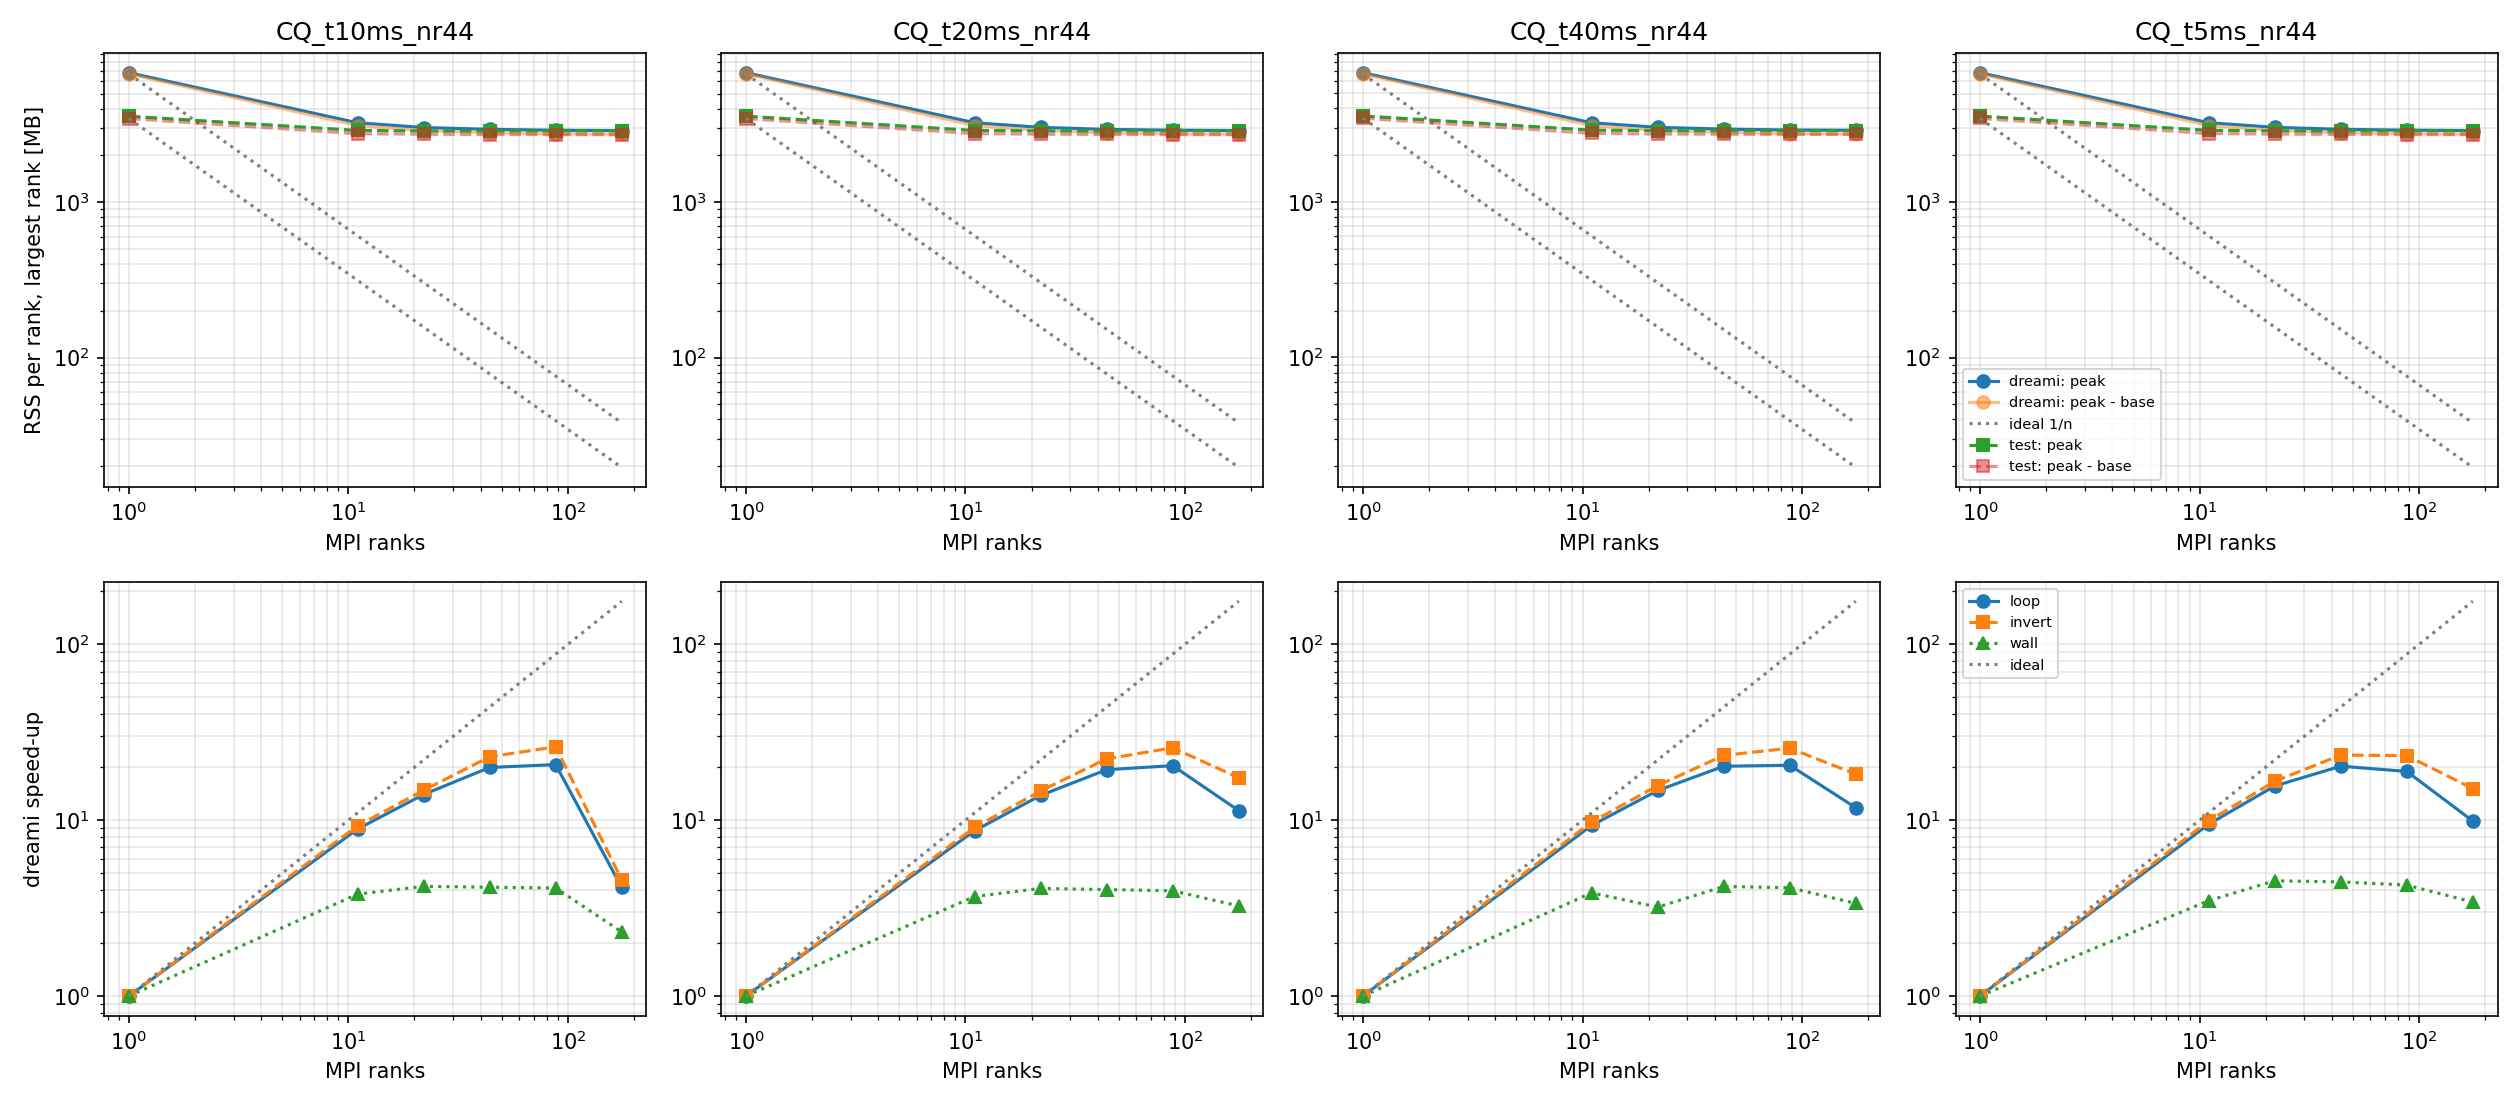
\includegraphics[width=0.92\linewidth]{v4_2900942/memory_scaling}
    \end{center}
    \vspace{-0.6em}
    \begin{columns}[T]
        \begin{column}{0.48\textwidth}
            \begin{itemize}
                \item top, peak memory per rank: 6.7\,GB (1) $\to$ 3.3\,GB (11) $\to$ 2.9\,GB (176):
                      \textbf{plateau at $\approx 2.9$\,GB}
            \end{itemize}
        \end{column}
        \begin{column}{0.48\textwidth}
            \begin{itemize}
                \item bottom, speed-up: linear solve 28.9\,s $\to$ 1.1\,s at 88 ranks ($\times 26$),
                      slower at 176; whole run 35.8\,s $\to$ 8.7\,s ($\times 4$)
            \end{itemize}
        \end{column}
    \end{columns}
\end{frame}

% ---------------------------------------------------------------------
\begin{frame}{Memory and time breakdown: toroidal geometry}
    \footnotesize
    \begin{center}
        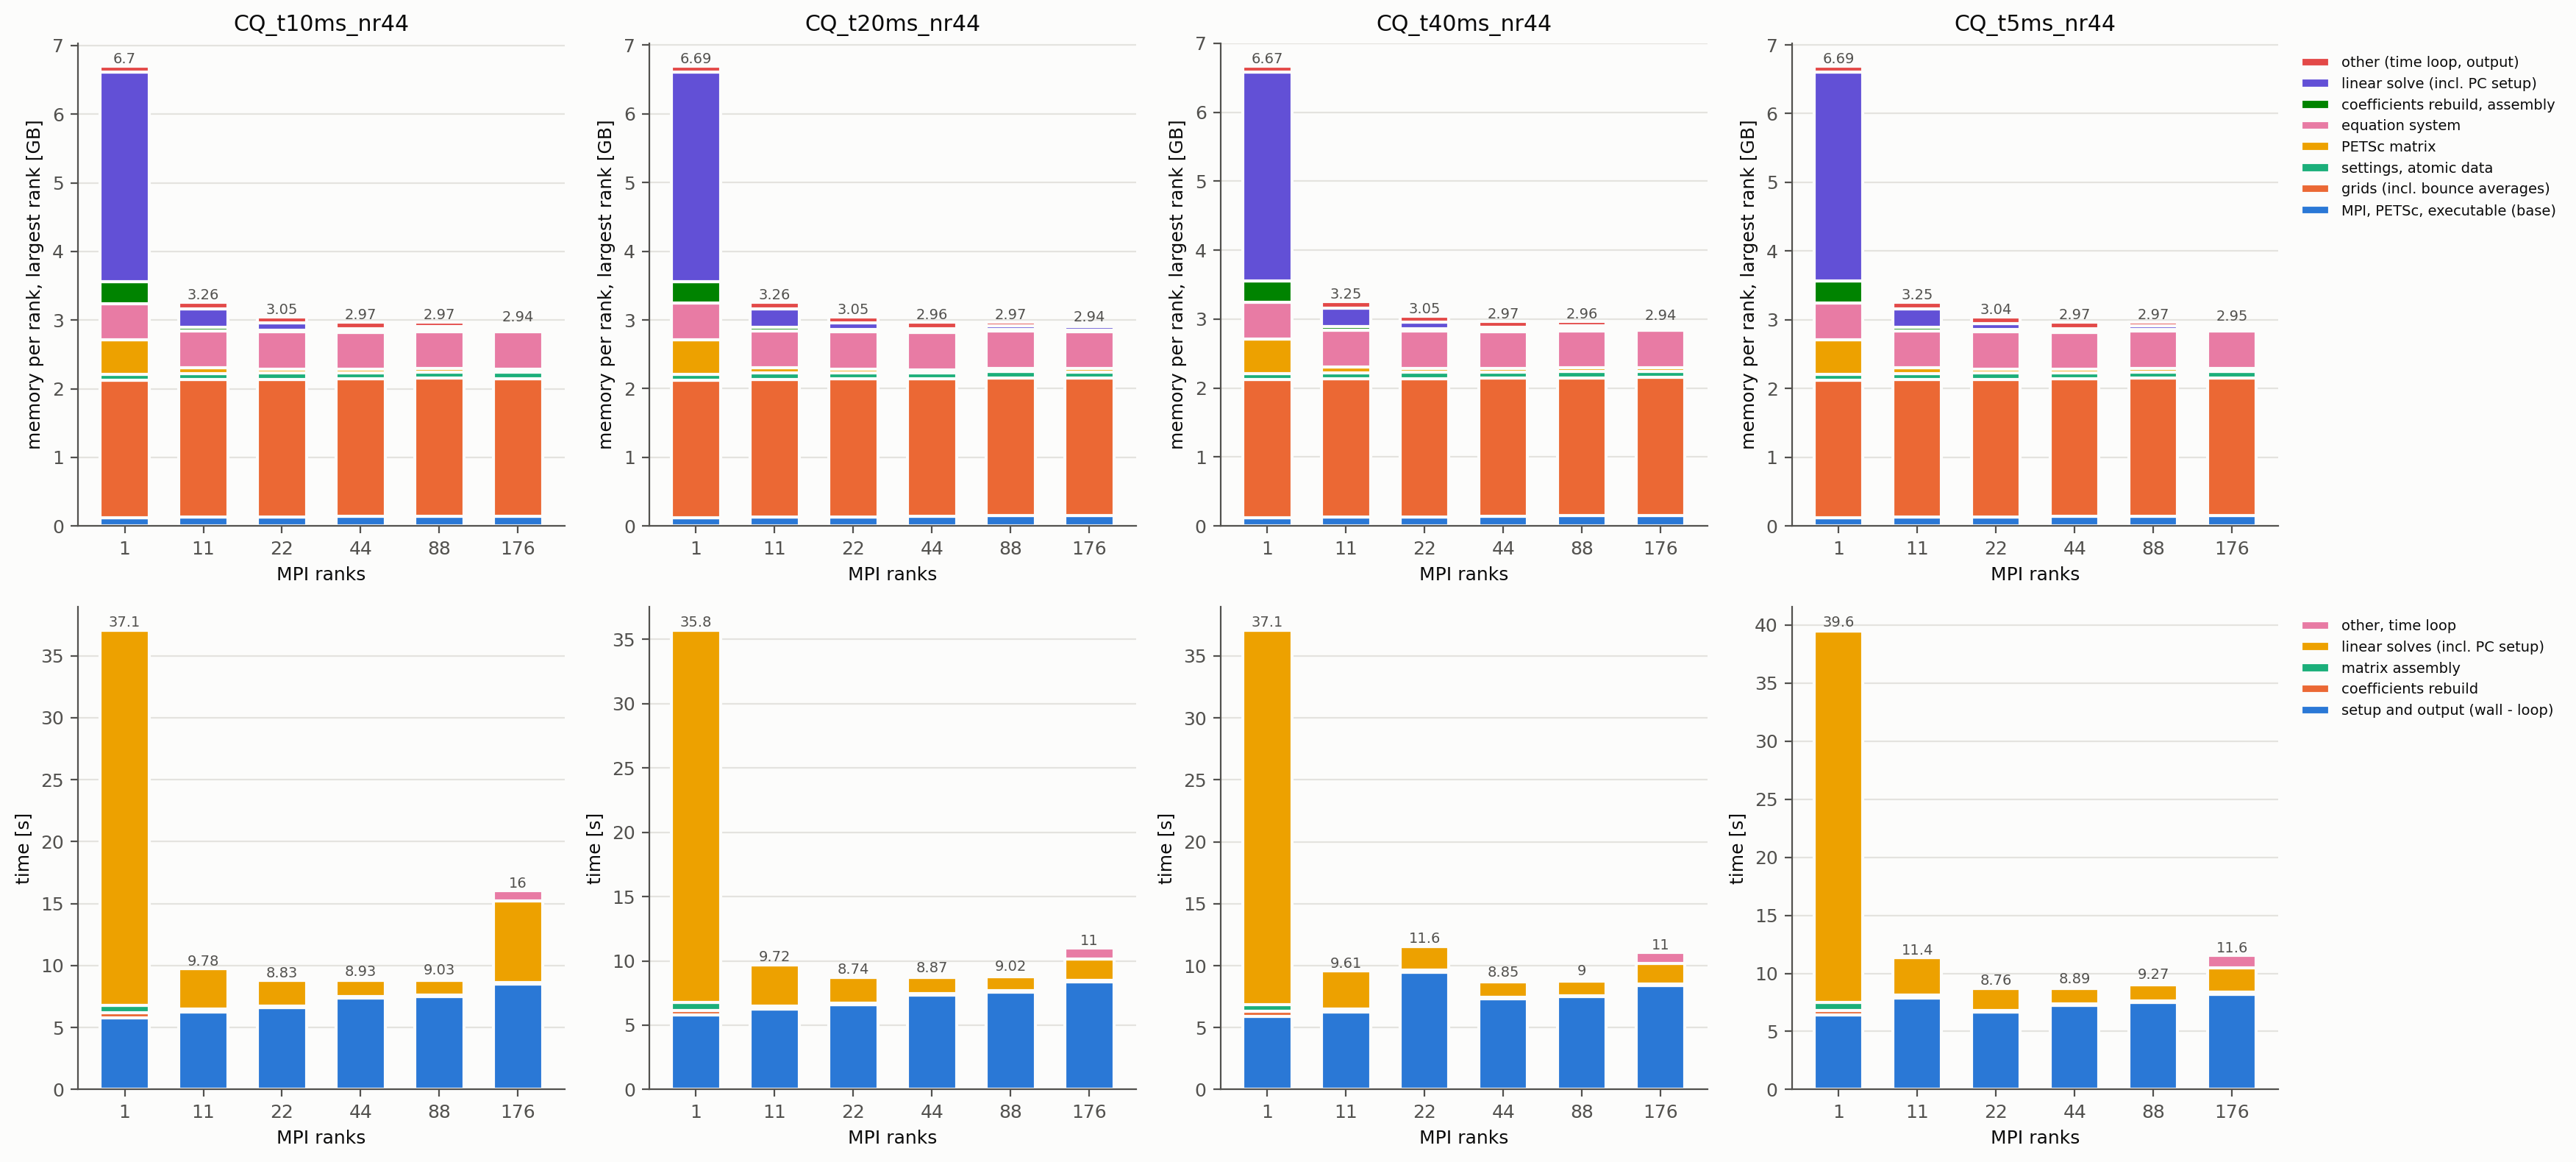
\includegraphics[width=0.92\linewidth]{v4_2900942/memory_time_breakdown}
    \end{center}
    \vspace{-0.6em}
    \begin{columns}[T]
        \begin{column}{0.48\textwidth}
            \begin{itemize}
                \item \textbf{distributed parts scale} (CQ 20\,ms, 1 $\to$ 176 ranks):
                      linear solve 3.1\,GB $\to$ 46\,MB, PETSc matrix 511 $\to$ 49\,MB
                \item \textbf{grids are replicated}: 2.05\,GB on every rank
                      (hot-tail 0.67, runaway 1.38\,GB, incl.\ bounce averages), 70\% of the plateau
            \end{itemize}
        \end{column}
        \begin{column}{0.48\textwidth}
            \begin{itemize}
                \item time: with $\geq 11$ ranks, setup and output
                      (6--8\,s, not parallel) dominate the run
                \item next: distribute the grid quantities by radius
            \end{itemize}
        \end{column}
    \end{columns}
\end{frame}
 (update_2026-11-24.tex).

% =====================================================================
% Part 1: linear solver
% =====================================================================
\begin{frame}{Linear solver comparison: setup}
    \small
    \begin{itemize}
        \item kinetic system dumped by \texttt{dreami} (\texttt{-dream\_save\_system}), L2, cylindrical
        \begin{itemize}
            \item $N = 1.67$\,M unknowns, $11.4$\,M nonzeros
            \item $N_r = 11$ radii, $152\,000$ rows per radius ($f_\mathrm{hot}$ $32\,000$ + $f_\mathrm{re}$ $120\,000$)
        \end{itemize}
        \item two snapshots
        \begin{itemize}
            \item injection end ($\Delta t = 1.8\times10^{-7}$\,s, the source step)
            \item current quench at 29\,ms, $E \approx 31$\,V/m, with
                  $\Delta t = 1.0\times10^{-7}$\,s, the DREAM substep of V.~Svensson's coupled runs
                  ($N_t = \lceil \Delta t_\mathrm{fluid} / 10^{-7}\,\mathrm{s} \rceil$),
                  instead of the source step $10^{-4}$\,s
        \end{itemize}
        \item serial, zero initial guess, restart 100, stop at $\|r\|/\|b\| < 10^{-10}$ (true residual)
        \item five solvers; ``BJ(r)'' = block Jacobi over the radius, one block per radius
        \begin{enumerate}
            \item BJ(r) + [GMRES + AMG with Euclid ILU(1) smoother] + FGMRES \quad (MIRadialBJ)
            \item BJ(r) + one AMG V-cycle + GMRES
            \item BJ(r) + ILU(0) + GMRES
            \item AMG + GMRES \quad (whole matrix)
            \item ILU(0) + GMRES \quad (whole matrix)
        \end{enumerate}
    \end{itemize}
\end{frame}

% ---------------------------------------------------------------------
\begin{frame}{Linear solver comparison: results (serial, L2)}
    \small
    \begin{center}
    \resizebox{\linewidth}{!}{%
    \begin{tabular}{l|rrr|rrr}
        \hline
        & \multicolumn{3}{c|}{injection end} & \multicolumn{3}{c}{CQ 29\,ms, $\Delta t = 10^{-7}$\,s} \\
        solver & its & time [s] & error & its & time [s] & error \\
        \hline
        \textbf{BJ(r) + [GMRES+AMG/Euclid(1)] + FGMRES} & \textbf{3} & \textbf{6.8} & $5\times10^{-12}$
                                                       & \textbf{3} & \textbf{4.7} & $4\times10^{-12}$ \\
        BJ(r) + AMG + GMRES        & 22  & 8.4  & $7\times10^{-11}$ & 221 & 41.3 & $1\times10^{-11}$ \\
        BJ(r) + ILU(0) + GMRES     & 152 & 29.4 & $1\times10^{-10}$ & 238 & 19.9 & $1\times10^{-10}$ \\
        AMG + GMRES                & 21  & 11.1 & $9\times10^{-12}$ & --  & --   & -- \\
        ILU(0) + GMRES             & 150 & 29.8 & $1\times10^{-10}$ & --  & --   & -- \\
        \hline
    \end{tabular}}
    \end{center}
    \vspace{0.3em}
    \begin{itemize}
        \item time = setup + solve; error = $\|x - x_\mathrm{ref}\| / \|x_\mathrm{ref}\|$
        \item method 1: inner GMRES at most 9 iterations per radius (99 in total), on both snapshots
        \item CQ, AMG + GMRES and ILU(0) + GMRES: out of memory on the serial partition, to be re-run
        \item true residual after ``convergence'': $\lesssim 10^{-9}$, except with AMG
              (BJ(r) + AMG: $7\times10^{-8}$, AMG: $1\times10^{-8}$)
    \end{itemize}
\end{frame}

% ---------------------------------------------------------------------
\begin{frame}{Chosen linear method}
    \begin{center}
        \textbf{FGMRES, preconditioned by block Jacobi over the radius;}\\
        \textbf{each block solved by GMRES + BoomerAMG with Euclid ILU(1) smoother}
    \end{center}
    \vspace{0.5em}
    \small
    \begin{itemize}
        \item \textbf{fewest iterations}: 3 outer iterations on both snapshots
        \item \textbf{fastest}: 4.7\,s (CQ) and 6.8\,s (injection);
              next best 19.9\,s (CQ, BJ + ILU) and 8.4\,s (injection, BJ + AMG)
        \item \textbf{robust}: BJ + one AMG V-cycle needs 22 iterations at injection but 221 in the CQ;
              method 1 needs 3 in both
        \item \textbf{parallel by construction}: one block per radius, so with up to $N_r$ ranks
              the preconditioner needs no communication; the radial coupling is left to the outer FGMRES
        \item FGMRES because the inner Krylov solve makes the preconditioner change from one iteration to the next
        \item Euclid ILU(1) rather than ILU(0): with ILU(0) the inner GMRES breaks down on
              some radii of the CQ snapshot at 29\,ms
    \end{itemize}
\end{frame}

% =====================================================================
% Part 2: memory and time scaling, toroidal geometry
% =====================================================================
\begin{frame}{Memory and speed-up test: toroidal geometry}
    \footnotesize
    4 CQ snapshots (5, 10, 20, 40\,ms), analytic toroidal geometry, L1, $N_r = 44$:
    1.67\,M unknowns, 1 time step, MIRadialBJ; same behaviour for the 4 snapshots
    \begin{center}
        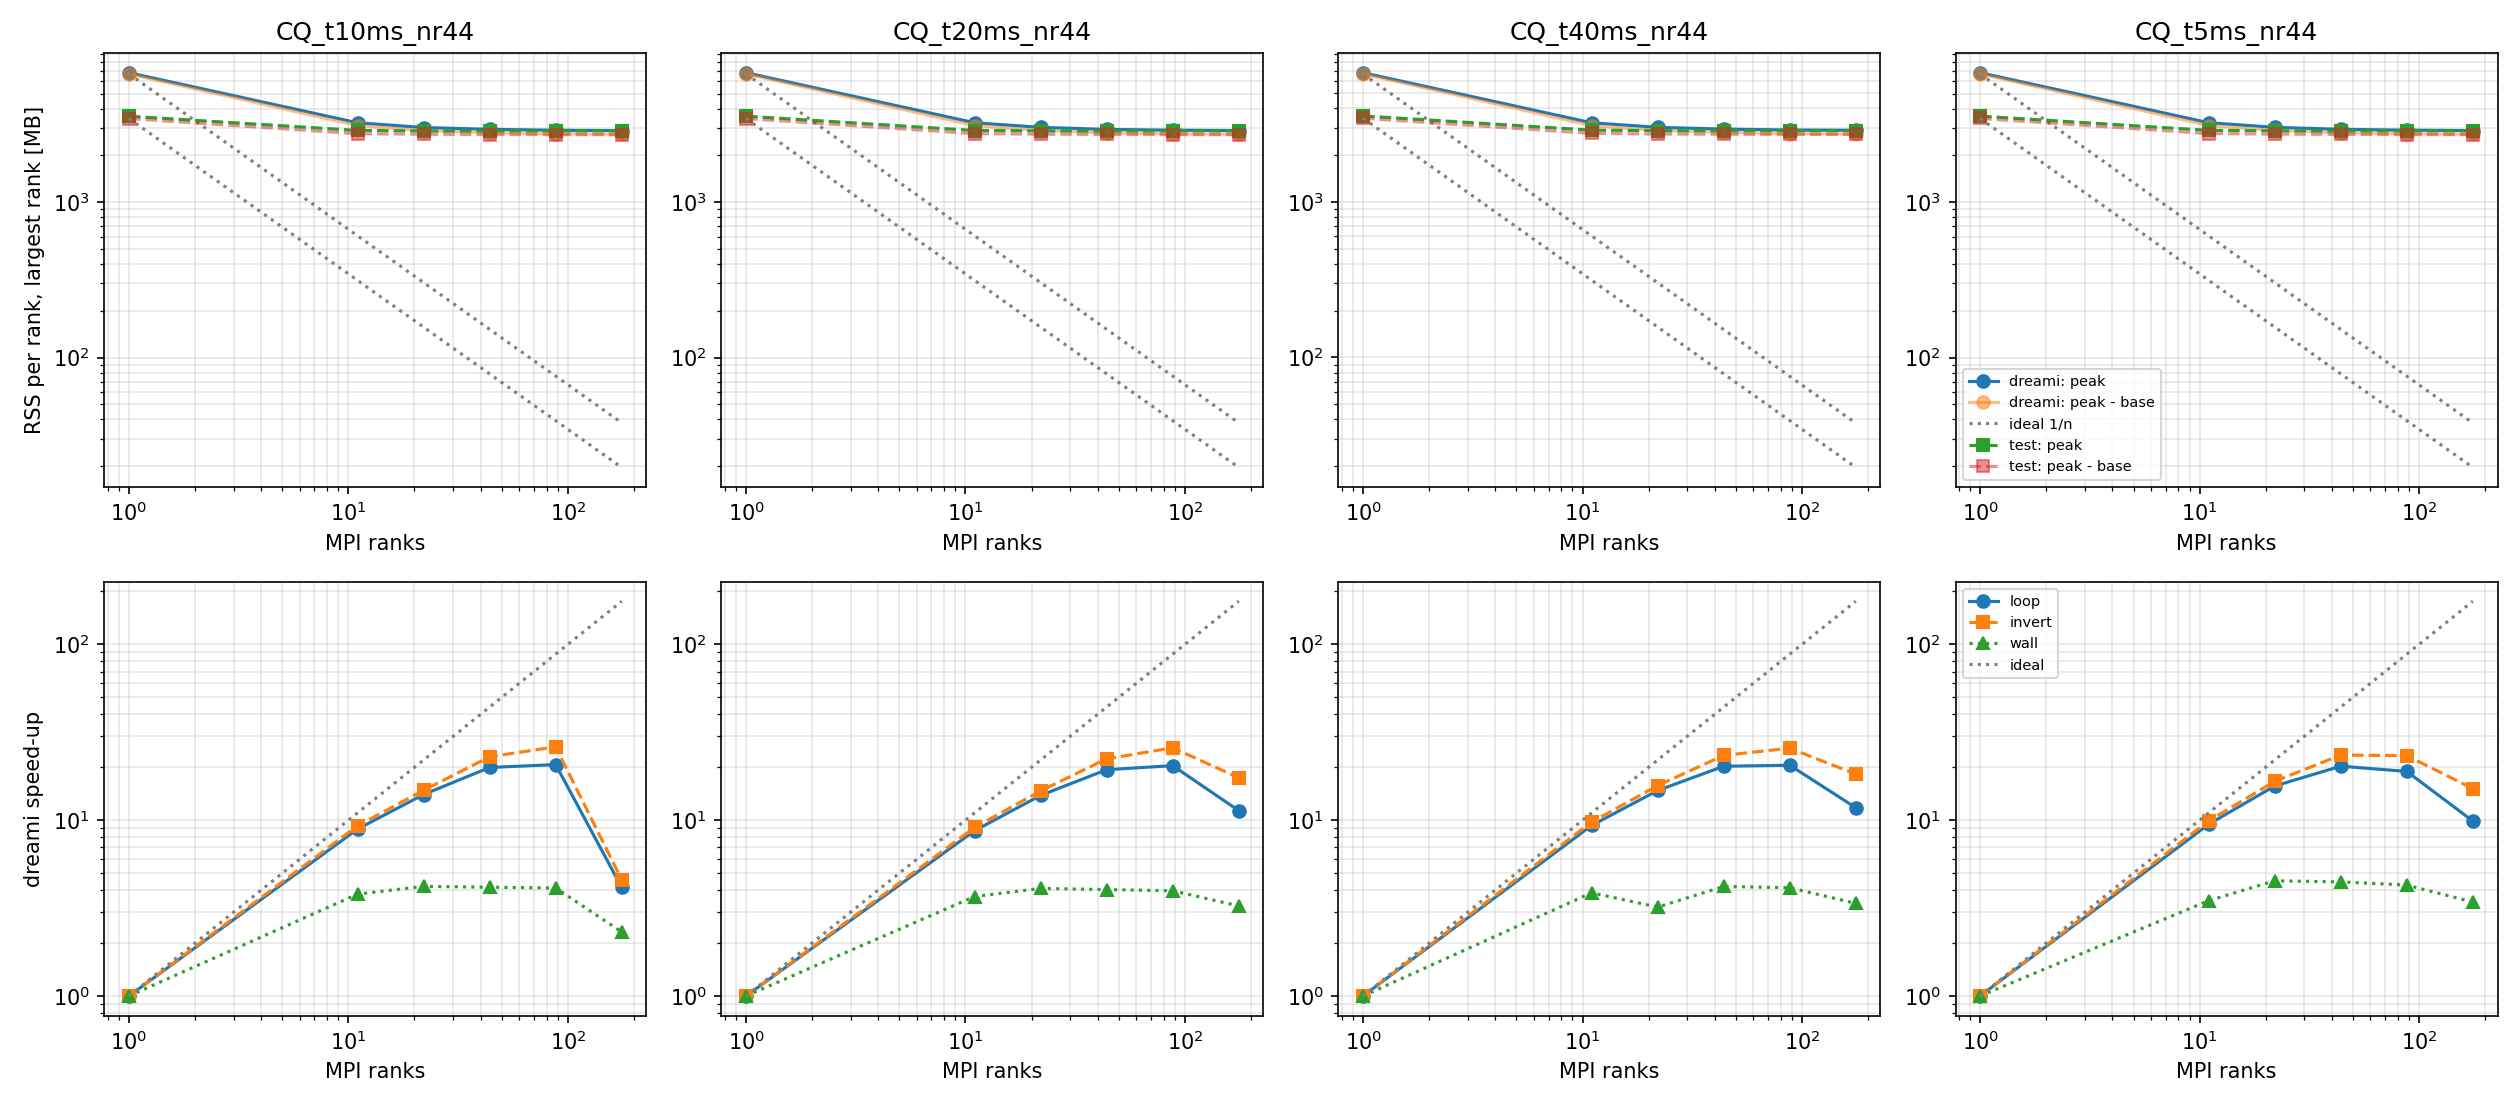
\includegraphics[width=0.92\linewidth]{v4_2900942/memory_scaling}
    \end{center}
    \vspace{-0.6em}
    \begin{columns}[T]
        \begin{column}{0.48\textwidth}
            \begin{itemize}
                \item top, peak memory per rank: 6.7\,GB (1) $\to$ 3.3\,GB (11) $\to$ 2.9\,GB (176):
                      \textbf{plateau at $\approx 2.9$\,GB}
            \end{itemize}
        \end{column}
        \begin{column}{0.48\textwidth}
            \begin{itemize}
                \item bottom, speed-up: linear solve 28.9\,s $\to$ 1.1\,s at 88 ranks ($\times 26$),
                      slower at 176; whole run 35.8\,s $\to$ 8.7\,s ($\times 4$)
            \end{itemize}
        \end{column}
    \end{columns}
\end{frame}

% ---------------------------------------------------------------------
\begin{frame}{Memory and time breakdown: toroidal geometry}
    \footnotesize
    \begin{center}
        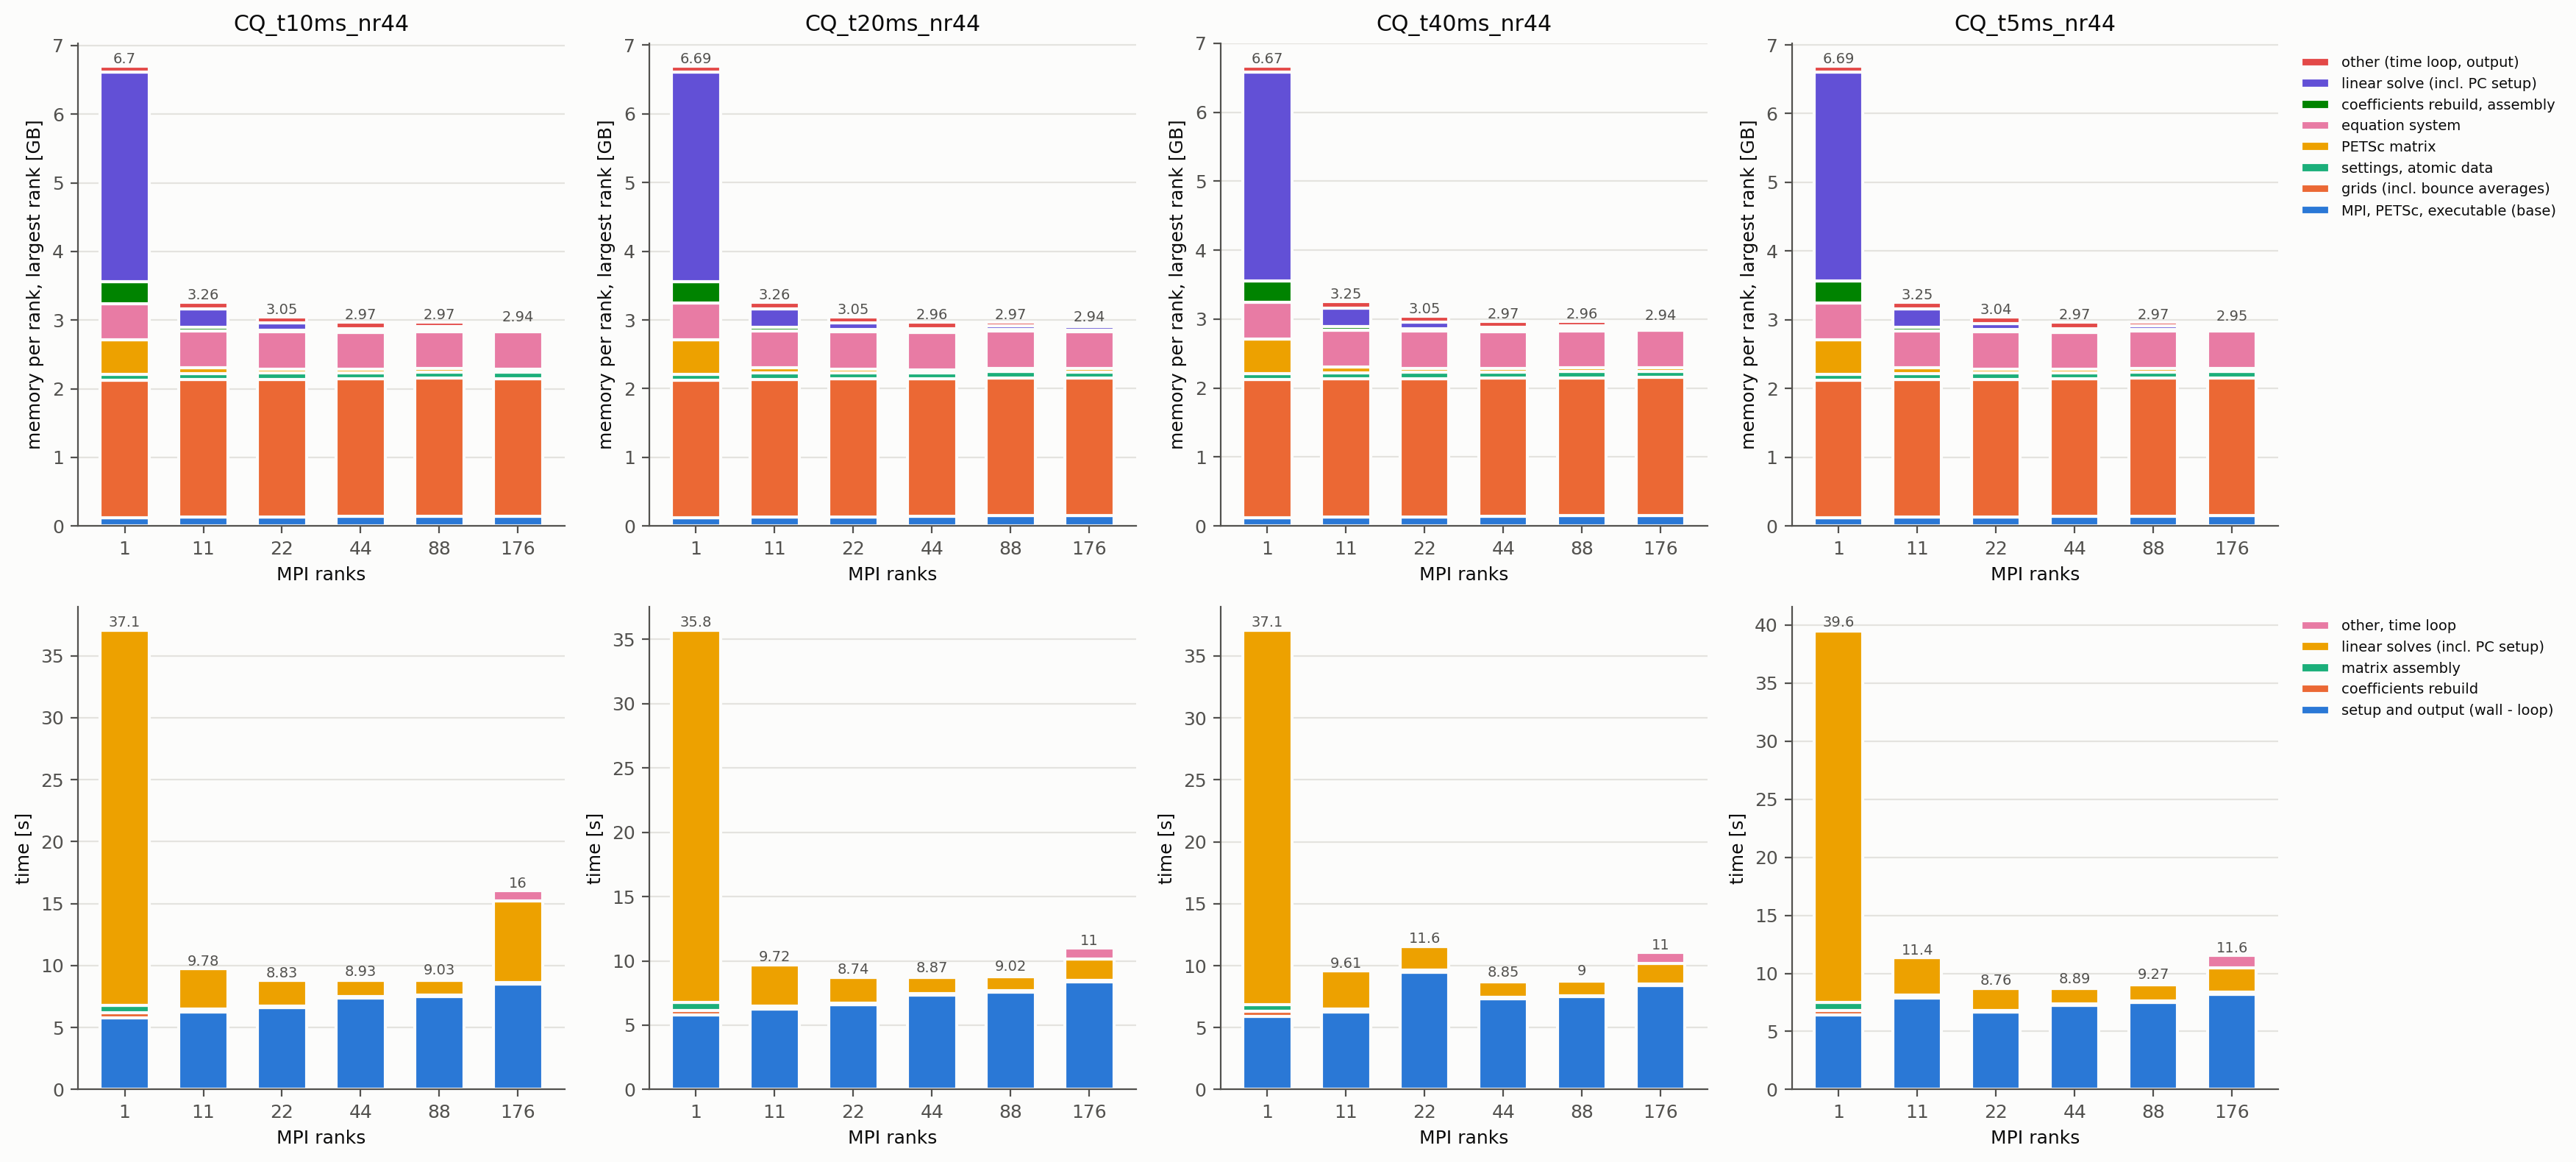
\includegraphics[width=0.92\linewidth]{v4_2900942/memory_time_breakdown}
    \end{center}
    \vspace{-0.6em}
    \begin{columns}[T]
        \begin{column}{0.48\textwidth}
            \begin{itemize}
                \item \textbf{distributed parts scale} (CQ 20\,ms, 1 $\to$ 176 ranks):
                      linear solve 3.1\,GB $\to$ 46\,MB, PETSc matrix 511 $\to$ 49\,MB
                \item \textbf{grids are replicated}: 2.05\,GB on every rank
                      (hot-tail 0.67, runaway 1.38\,GB, incl.\ bounce averages), 70\% of the plateau
            \end{itemize}
        \end{column}
        \begin{column}{0.48\textwidth}
            \begin{itemize}
                \item time: with $\geq 11$ ranks, setup and output
                      (6--8\,s, not parallel) dominate the run
                \item next: distribute the grid quantities by radius
            \end{itemize}
        \end{column}
    \end{columns}
\end{frame}
 (update_2026-11-24.tex).

% =====================================================================
% Part 1: linear solver
% =====================================================================
\begin{frame}{Linear solver comparison: setup}
    \small
    \begin{itemize}
        \item kinetic system dumped by \texttt{dreami} (\texttt{-dream\_save\_system}), L2, cylindrical
        \begin{itemize}
            \item $N = 1.67$\,M unknowns, $11.4$\,M nonzeros
            \item $N_r = 11$ radii, $152\,000$ rows per radius ($f_\mathrm{hot}$ $32\,000$ + $f_\mathrm{re}$ $120\,000$)
        \end{itemize}
        \item two snapshots
        \begin{itemize}
            \item injection end ($\Delta t = 1.8\times10^{-7}$\,s, the source step)
            \item current quench at 29\,ms, $E \approx 31$\,V/m, with
                  $\Delta t = 1.0\times10^{-7}$\,s, the DREAM substep of V.~Svensson's coupled runs
                  ($N_t = \lceil \Delta t_\mathrm{fluid} / 10^{-7}\,\mathrm{s} \rceil$),
                  instead of the source step $10^{-4}$\,s
        \end{itemize}
        \item serial, zero initial guess, restart 100, stop at $\|r\|/\|b\| < 10^{-10}$ (true residual)
        \item five solvers; ``BJ(r)'' = block Jacobi over the radius, one block per radius
        \begin{enumerate}
            \item BJ(r) + [GMRES + AMG with Euclid ILU(1) smoother] + FGMRES \quad (MIRadialBJ)
            \item BJ(r) + one AMG V-cycle + GMRES
            \item BJ(r) + ILU(0) + GMRES
            \item AMG + GMRES \quad (whole matrix)
            \item ILU(0) + GMRES \quad (whole matrix)
        \end{enumerate}
    \end{itemize}
\end{frame}

% ---------------------------------------------------------------------
\begin{frame}{Linear solver comparison: results (serial, L2)}
    \small
    \begin{center}
    \resizebox{\linewidth}{!}{%
    \begin{tabular}{l|rrr|rrr}
        \hline
        & \multicolumn{3}{c|}{injection end} & \multicolumn{3}{c}{CQ 29\,ms, $\Delta t = 10^{-7}$\,s} \\
        solver & its & time [s] & error & its & time [s] & error \\
        \hline
        \textbf{BJ(r) + [GMRES+AMG/Euclid(1)] + FGMRES} & \textbf{3} & \textbf{6.8} & $5\times10^{-12}$
                                                       & \textbf{3} & \textbf{4.7} & $4\times10^{-12}$ \\
        BJ(r) + AMG + GMRES        & 22  & 8.4  & $7\times10^{-11}$ & 221 & 41.3 & $1\times10^{-11}$ \\
        BJ(r) + ILU(0) + GMRES     & 152 & 29.4 & $1\times10^{-10}$ & 238 & 19.9 & $1\times10^{-10}$ \\
        AMG + GMRES                & 21  & 11.1 & $9\times10^{-12}$ & --  & --   & -- \\
        ILU(0) + GMRES             & 150 & 29.8 & $1\times10^{-10}$ & --  & --   & -- \\
        \hline
    \end{tabular}}
    \end{center}
    \vspace{0.3em}
    \begin{itemize}
        \item time = setup + solve; error = $\|x - x_\mathrm{ref}\| / \|x_\mathrm{ref}\|$
        \item method 1: inner GMRES at most 9 iterations per radius (99 in total), on both snapshots
        \item CQ, AMG + GMRES and ILU(0) + GMRES: out of memory on the serial partition, to be re-run
        \item true residual after ``convergence'': $\lesssim 10^{-9}$, except with AMG
              (BJ(r) + AMG: $7\times10^{-8}$, AMG: $1\times10^{-8}$)
    \end{itemize}
\end{frame}

% ---------------------------------------------------------------------
\begin{frame}{Chosen linear method}
    \begin{center}
        \textbf{FGMRES, preconditioned by block Jacobi over the radius;}\\
        \textbf{each block solved by GMRES + BoomerAMG with Euclid ILU(1) smoother}
    \end{center}
    \vspace{0.5em}
    \small
    \begin{itemize}
        \item \textbf{fewest iterations}: 3 outer iterations on both snapshots
        \item \textbf{fastest}: 4.7\,s (CQ) and 6.8\,s (injection);
              next best 19.9\,s (CQ, BJ + ILU) and 8.4\,s (injection, BJ + AMG)
        \item \textbf{robust}: BJ + one AMG V-cycle needs 22 iterations at injection but 221 in the CQ;
              method 1 needs 3 in both
        \item \textbf{parallel by construction}: one block per radius, so with up to $N_r$ ranks
              the preconditioner needs no communication; the radial coupling is left to the outer FGMRES
        \item FGMRES because the inner Krylov solve makes the preconditioner change from one iteration to the next
        \item Euclid ILU(1) rather than ILU(0): with ILU(0) the inner GMRES breaks down on
              some radii of the CQ snapshot at 29\,ms
    \end{itemize}
\end{frame}

% =====================================================================
% Part 2: memory and time scaling, toroidal geometry
% =====================================================================
\begin{frame}{Memory and speed-up test: toroidal geometry}
    \footnotesize
    4 CQ snapshots (5, 10, 20, 40\,ms), analytic toroidal geometry, L1, $N_r = 44$:
    1.67\,M unknowns, 1 time step, MIRadialBJ; same behaviour for the 4 snapshots
    \begin{center}
        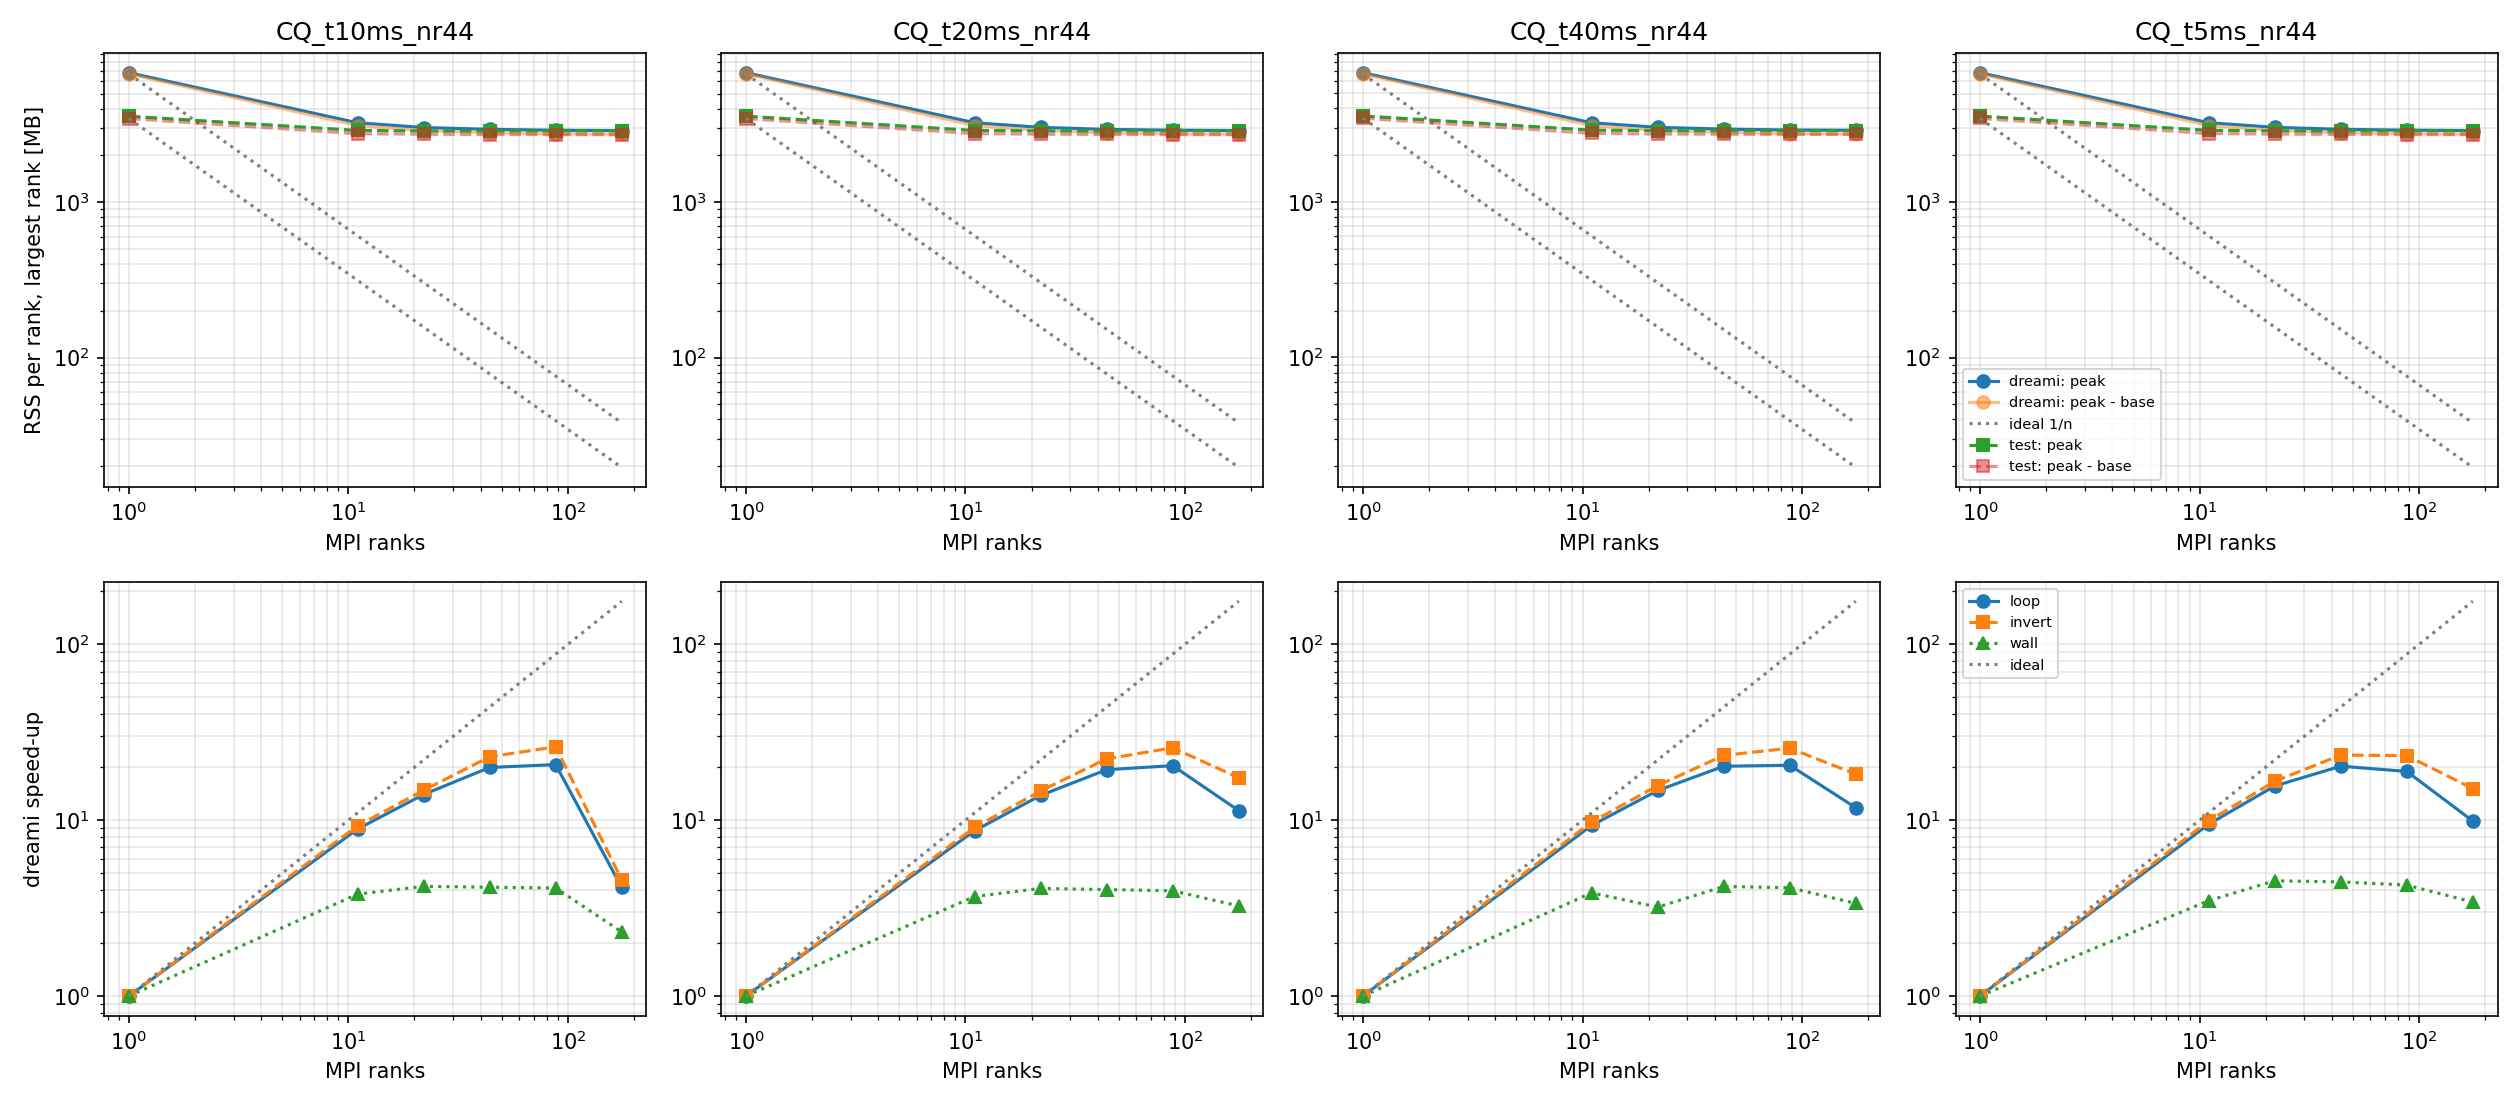
\includegraphics[width=0.92\linewidth]{v4_2900942/memory_scaling}
    \end{center}
    \vspace{-0.6em}
    \begin{columns}[T]
        \begin{column}{0.48\textwidth}
            \begin{itemize}
                \item top, peak memory per rank: 6.7\,GB (1) $\to$ 3.3\,GB (11) $\to$ 2.9\,GB (176):
                      \textbf{plateau at $\approx 2.9$\,GB}
            \end{itemize}
        \end{column}
        \begin{column}{0.48\textwidth}
            \begin{itemize}
                \item bottom, speed-up: linear solve 28.9\,s $\to$ 1.1\,s at 88 ranks ($\times 26$),
                      slower at 176; whole run 35.8\,s $\to$ 8.7\,s ($\times 4$)
            \end{itemize}
        \end{column}
    \end{columns}
\end{frame}

% ---------------------------------------------------------------------
\begin{frame}{Memory and time breakdown: toroidal geometry}
    \footnotesize
    \begin{center}
        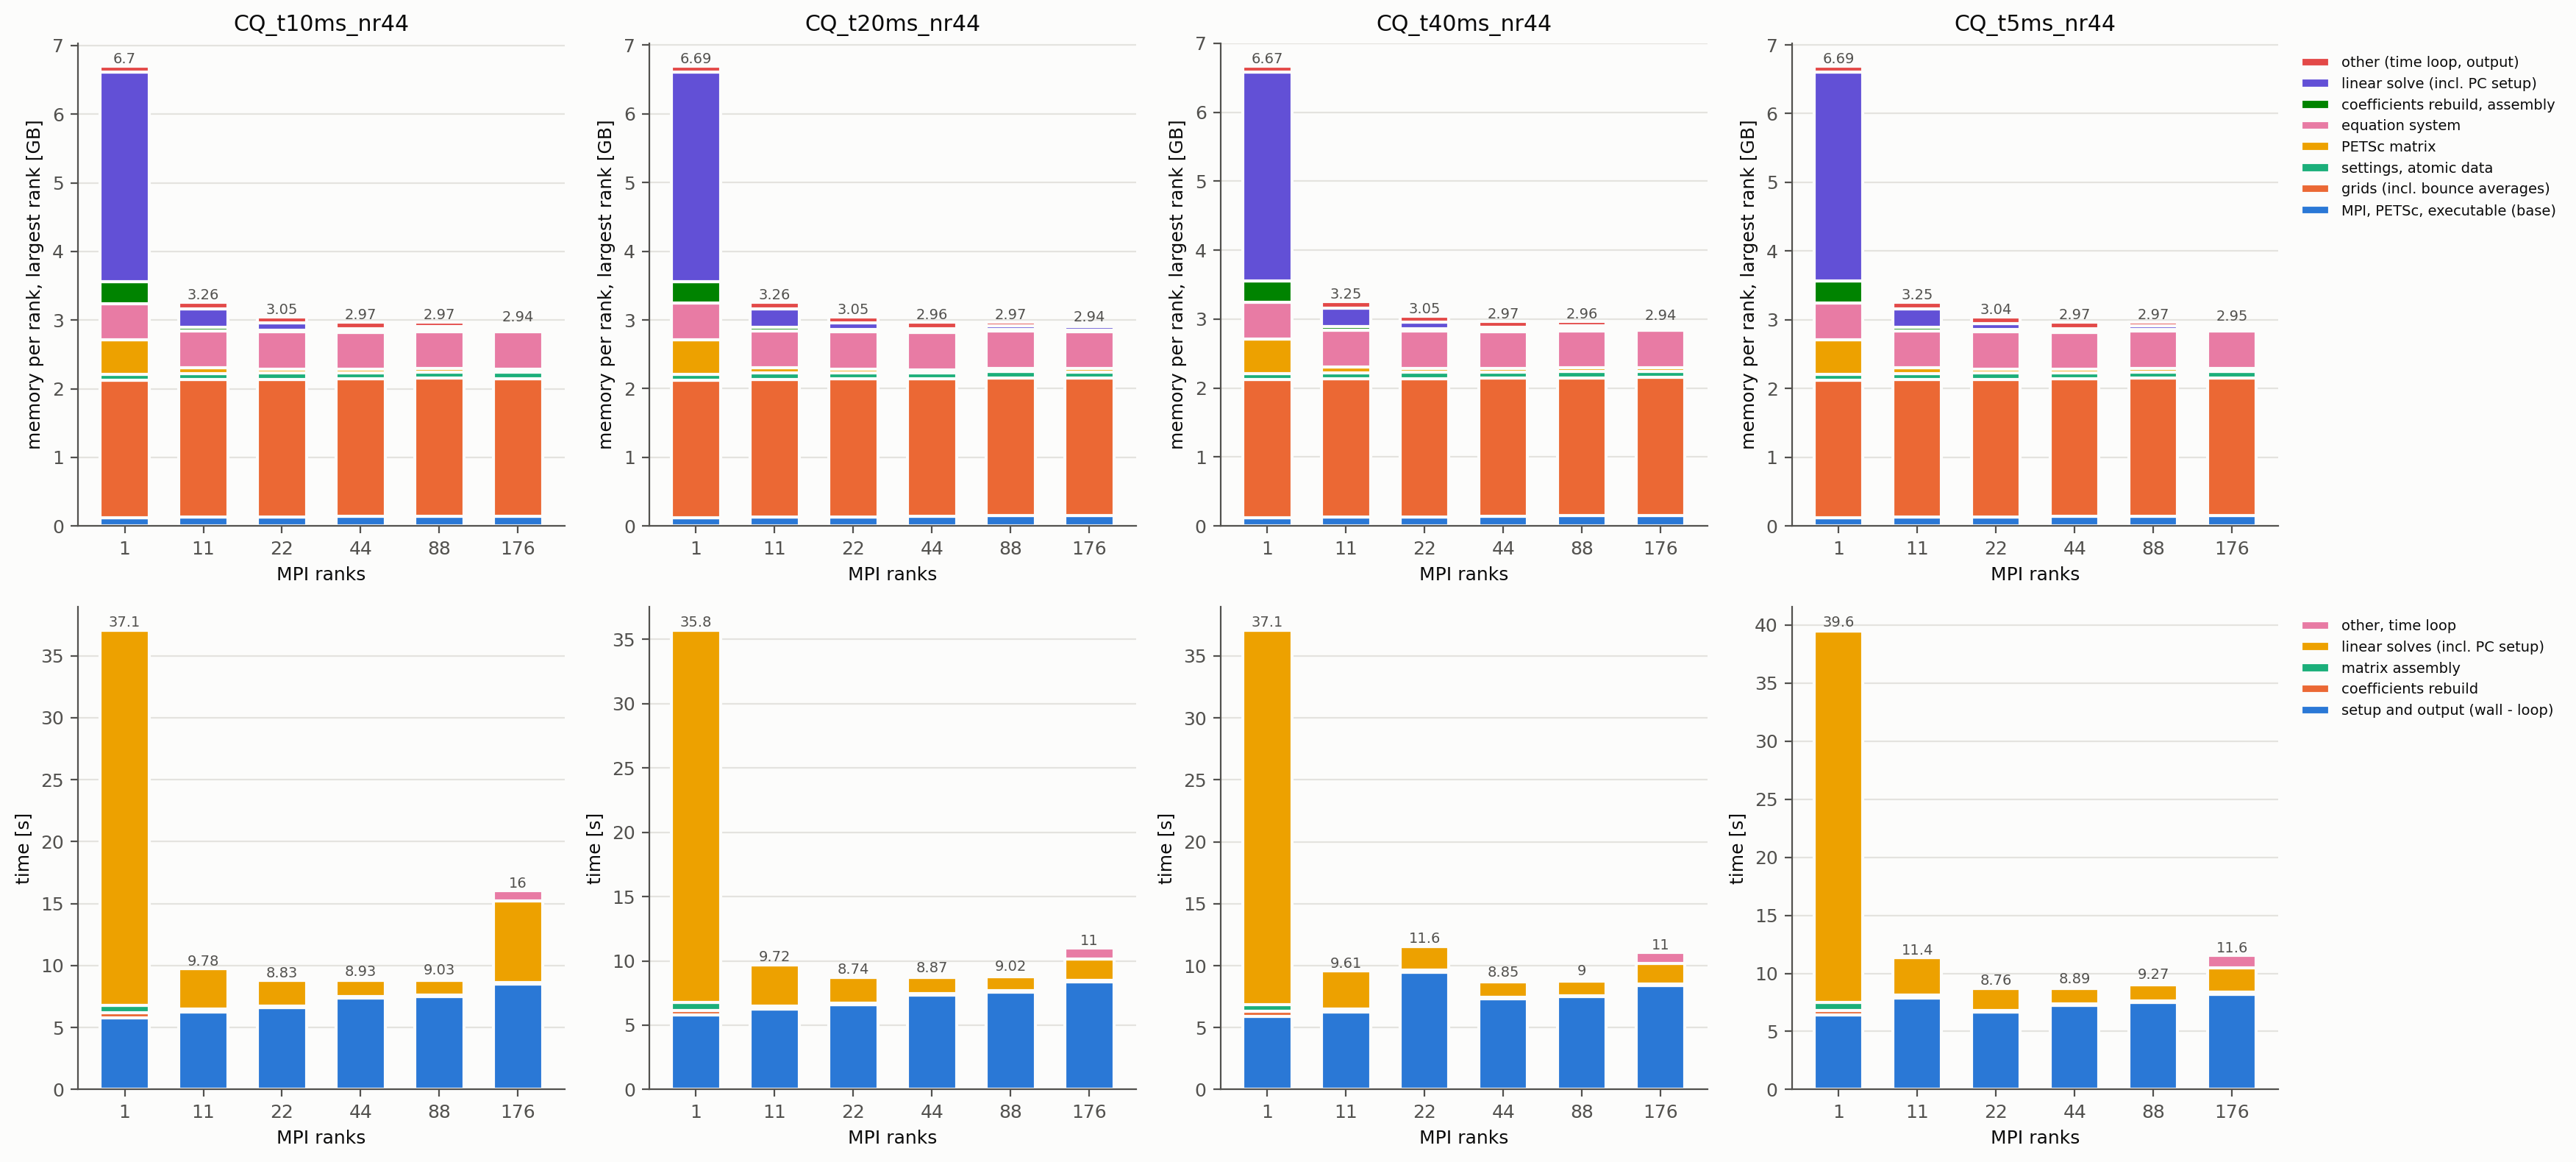
\includegraphics[width=0.92\linewidth]{v4_2900942/memory_time_breakdown}
    \end{center}
    \vspace{-0.6em}
    \begin{columns}[T]
        \begin{column}{0.48\textwidth}
            \begin{itemize}
                \item \textbf{distributed parts scale} (CQ 20\,ms, 1 $\to$ 176 ranks):
                      linear solve 3.1\,GB $\to$ 46\,MB, PETSc matrix 511 $\to$ 49\,MB
                \item \textbf{grids are replicated}: 2.05\,GB on every rank
                      (hot-tail 0.67, runaway 1.38\,GB, incl.\ bounce averages), 70\% of the plateau
            \end{itemize}
        \end{column}
        \begin{column}{0.48\textwidth}
            \begin{itemize}
                \item time: with $\geq 11$ ranks, setup and output
                      (6--8\,s, not parallel) dominate the run
                \item next: distribute the grid quantities by radius
            \end{itemize}
        \end{column}
    \end{columns}
\end{frame}
 (update_2026-11-24.tex).

% =====================================================================
% Part 1: linear solver
% =====================================================================
\begin{frame}{Linear solver comparison: setup}
    \small
    \begin{itemize}
        \item kinetic system dumped by \texttt{dreami} (\texttt{-dream\_save\_system}), L2, cylindrical
        \begin{itemize}
            \item $N = 1.67$\,M unknowns, $11.4$\,M nonzeros
            \item $N_r = 11$ radii, $152\,000$ rows per radius ($f_\mathrm{hot}$ $32\,000$ + $f_\mathrm{re}$ $120\,000$)
        \end{itemize}
        \item two snapshots
        \begin{itemize}
            \item injection end ($\Delta t = 1.8\times10^{-7}$\,s, the source step)
            \item current quench at 29\,ms, $E \approx 31$\,V/m, with
                  $\Delta t = 1.0\times10^{-7}$\,s, the DREAM substep of V.~Svensson's coupled runs
                  ($N_t = \lceil \Delta t_\mathrm{fluid} / 10^{-7}\,\mathrm{s} \rceil$),
                  instead of the source step $10^{-4}$\,s
        \end{itemize}
        \item serial, zero initial guess, restart 100, stop at $\|r\|/\|b\| < 10^{-10}$ (true residual)
        \item five solvers; ``BJ(r)'' = block Jacobi over the radius, one block per radius
        \begin{enumerate}
            \item BJ(r) + [GMRES + AMG with Euclid ILU(1) smoother] + FGMRES \quad (MIRadialBJ)
            \item BJ(r) + one AMG V-cycle + GMRES
            \item BJ(r) + ILU(0) + GMRES
            \item AMG + GMRES \quad (whole matrix)
            \item ILU(0) + GMRES \quad (whole matrix)
        \end{enumerate}
    \end{itemize}
\end{frame}

% ---------------------------------------------------------------------
\begin{frame}{Linear solver comparison: results (serial, L2)}
    \small
    \begin{center}
    \resizebox{\linewidth}{!}{%
    \begin{tabular}{l|rrr|rrr}
        \hline
        & \multicolumn{3}{c|}{injection end} & \multicolumn{3}{c}{CQ 29\,ms, $\Delta t = 10^{-7}$\,s} \\
        solver & its & time [s] & error & its & time [s] & error \\
        \hline
        \textbf{BJ(r) + [GMRES+AMG/Euclid(1)] + FGMRES} & \textbf{3} & \textbf{6.8} & $5\times10^{-12}$
                                                       & \textbf{3} & \textbf{4.7} & $4\times10^{-12}$ \\
        BJ(r) + AMG + GMRES        & 22  & 8.4  & $7\times10^{-11}$ & 221 & 41.3 & $1\times10^{-11}$ \\
        BJ(r) + ILU(0) + GMRES     & 152 & 29.4 & $1\times10^{-10}$ & 238 & 19.9 & $1\times10^{-10}$ \\
        AMG + GMRES                & 21  & 11.1 & $9\times10^{-12}$ & --  & --   & -- \\
        ILU(0) + GMRES             & 150 & 29.8 & $1\times10^{-10}$ & --  & --   & -- \\
        \hline
    \end{tabular}}
    \end{center}
    \vspace{0.3em}
    \begin{itemize}
        \item time = setup + solve; error = $\|x - x_\mathrm{ref}\| / \|x_\mathrm{ref}\|$
        \item method 1: inner GMRES at most 9 iterations per radius (99 in total), on both snapshots
        \item CQ, AMG + GMRES and ILU(0) + GMRES: out of memory on the serial partition, to be re-run
        \item true residual after ``convergence'': $\lesssim 10^{-9}$, except with AMG
              (BJ(r) + AMG: $7\times10^{-8}$, AMG: $1\times10^{-8}$)
    \end{itemize}
\end{frame}

% ---------------------------------------------------------------------
\begin{frame}{Chosen linear method}
    \begin{center}
        \textbf{FGMRES, preconditioned by block Jacobi over the radius;}\\
        \textbf{each block solved by GMRES + BoomerAMG with Euclid ILU(1) smoother}
    \end{center}
    \vspace{0.5em}
    \small
    \begin{itemize}
        \item \textbf{fewest iterations}: 3 outer iterations on both snapshots
        \item \textbf{fastest}: 4.7\,s (CQ) and 6.8\,s (injection);
              next best 19.9\,s (CQ, BJ + ILU) and 8.4\,s (injection, BJ + AMG)
        \item \textbf{robust}: BJ + one AMG V-cycle needs 22 iterations at injection but 221 in the CQ;
              method 1 needs 3 in both
        \item \textbf{parallel by construction}: one block per radius, so with up to $N_r$ ranks
              the preconditioner needs no communication; the radial coupling is left to the outer FGMRES
        \item FGMRES because the inner Krylov solve makes the preconditioner change from one iteration to the next
        \item Euclid ILU(1) rather than ILU(0): with ILU(0) the inner GMRES breaks down on
              some radii of the CQ snapshot at 29\,ms
    \end{itemize}
\end{frame}

% =====================================================================
% Part 2: memory and time scaling, toroidal geometry
% =====================================================================
\begin{frame}{Memory and speed-up test: toroidal geometry}
    \footnotesize
    4 CQ snapshots (5, 10, 20, 40\,ms), analytic toroidal geometry, L1, $N_r = 44$:
    1.67\,M unknowns, 1 time step, MIRadialBJ; same behaviour for the 4 snapshots
    \begin{center}
        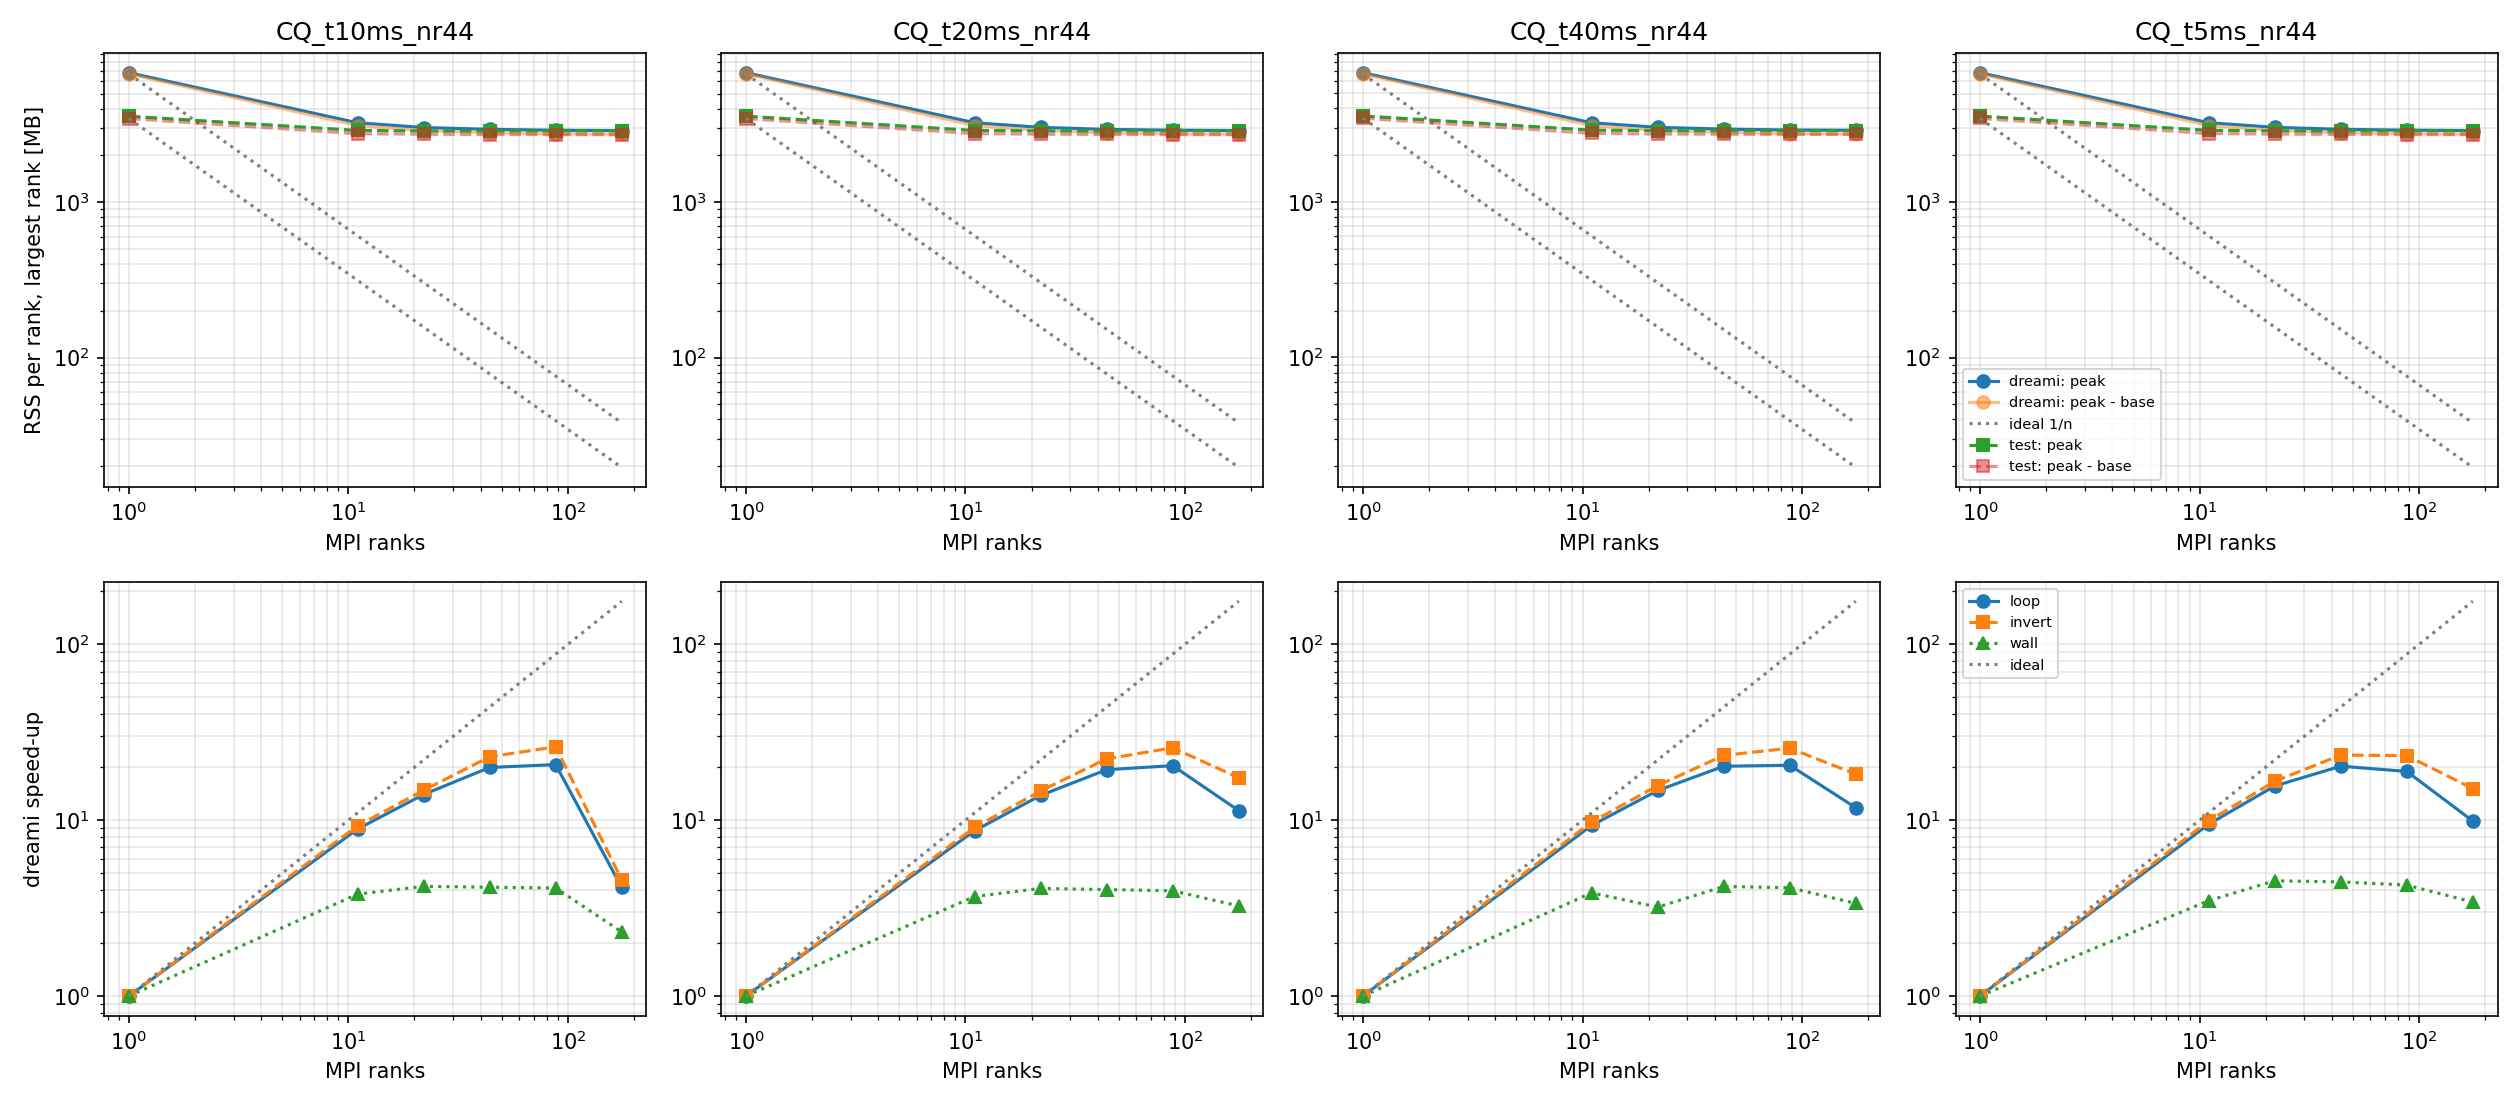
\includegraphics[width=0.92\linewidth]{v4_2900942/memory_scaling}
    \end{center}
    \vspace{-0.6em}
    \begin{columns}[T]
        \begin{column}{0.48\textwidth}
            \begin{itemize}
                \item top, peak memory per rank: 6.7\,GB (1) $\to$ 3.3\,GB (11) $\to$ 2.9\,GB (176):
                      \textbf{plateau at $\approx 2.9$\,GB}
            \end{itemize}
        \end{column}
        \begin{column}{0.48\textwidth}
            \begin{itemize}
                \item bottom, speed-up: linear solve 28.9\,s $\to$ 1.1\,s at 88 ranks ($\times 26$),
                      slower at 176; whole run 35.8\,s $\to$ 8.7\,s ($\times 4$)
            \end{itemize}
        \end{column}
    \end{columns}
\end{frame}

% ---------------------------------------------------------------------
\begin{frame}{Memory and time breakdown: toroidal geometry}
    \footnotesize
    \begin{center}
        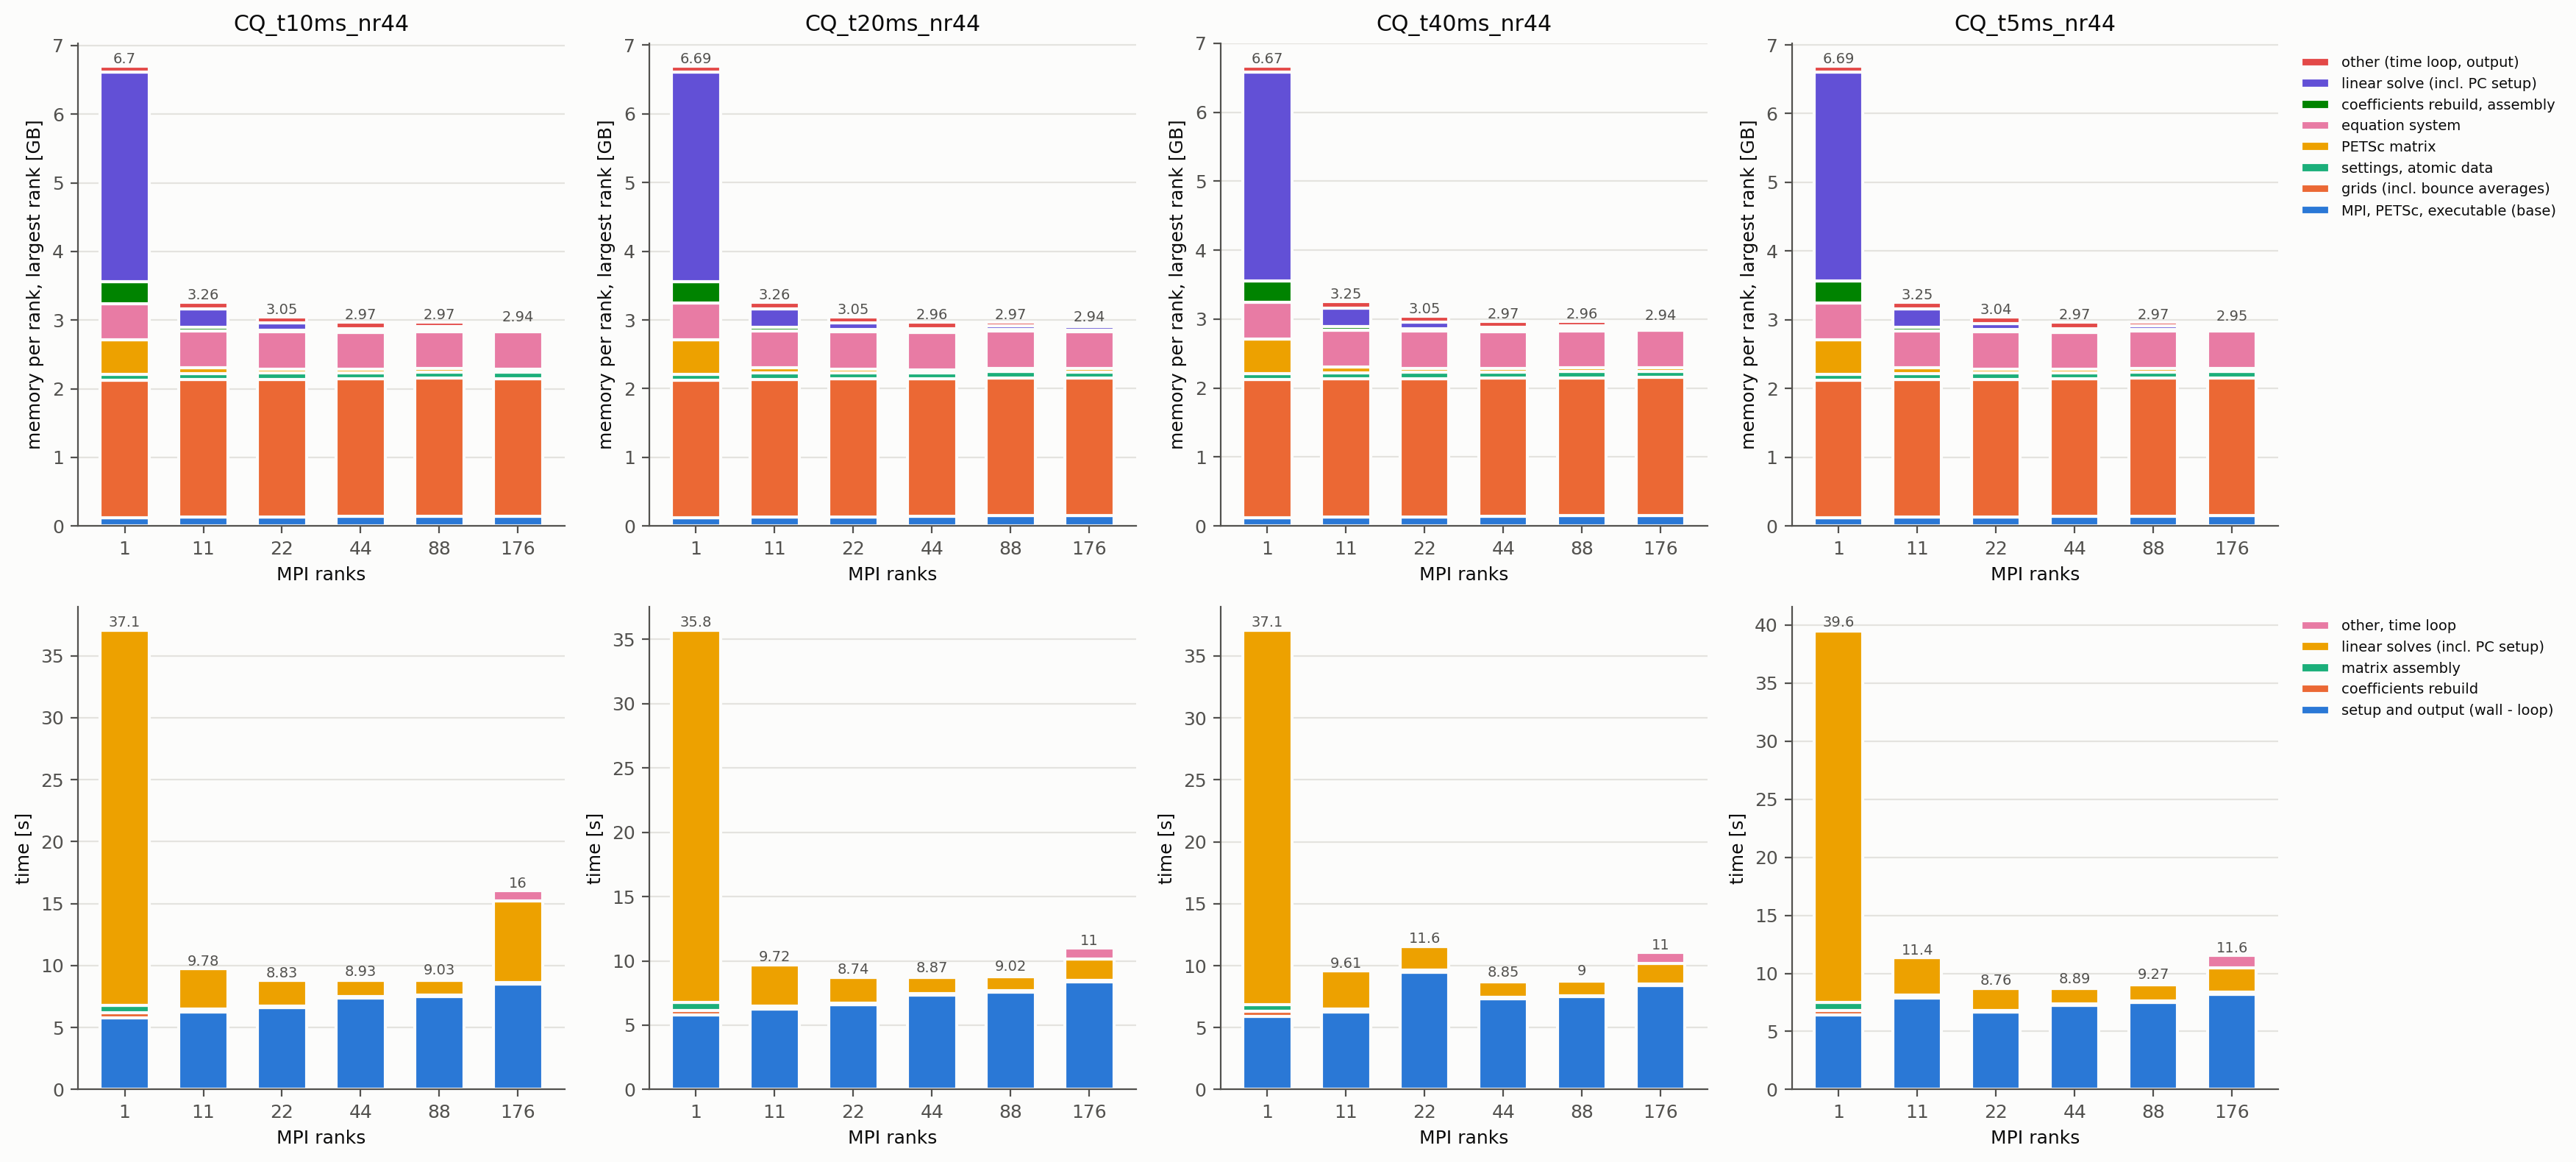
\includegraphics[width=0.92\linewidth]{v4_2900942/memory_time_breakdown}
    \end{center}
    \vspace{-0.6em}
    \begin{columns}[T]
        \begin{column}{0.48\textwidth}
            \begin{itemize}
                \item \textbf{distributed parts scale} (CQ 20\,ms, 1 $\to$ 176 ranks):
                      linear solve 3.1\,GB $\to$ 46\,MB, PETSc matrix 511 $\to$ 49\,MB
                \item \textbf{grids are replicated}: 2.05\,GB on every rank
                      (hot-tail 0.67, runaway 1.38\,GB, incl.\ bounce averages), 70\% of the plateau
            \end{itemize}
        \end{column}
        \begin{column}{0.48\textwidth}
            \begin{itemize}
                \item time: with $\geq 11$ ranks, setup and output
                      (6--8\,s, not parallel) dominate the run
                \item next: distribute the grid quantities by radius
            \end{itemize}
        \end{column}
    \end{columns}
\end{frame}
